% TASK58_DRAFT_STUB
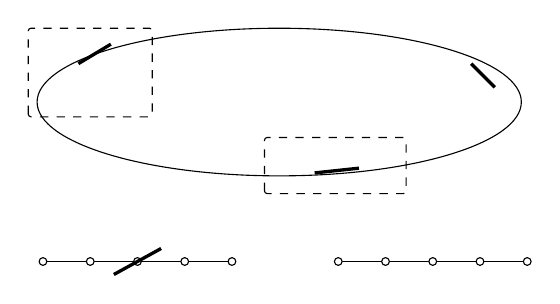
\begin{tikzpicture}[
  x=0.75cm,
  y=0.75cm,
  ring/.style={draw=black,thin},
  core/.style={draw=black,line width=1.2pt},
  support/.style={draw=black,dashed,rounded corners=1pt},
  patch/.style={draw=black,thin}
]
  \draw[ring] (0,2.3) ellipse (4.1 and 1.25);
  \draw[core] (-3.4,2.95)--(-2.85,3.28);
  \draw[core] (0.6,1.1)--(1.35,1.18);
  \draw[core] (3.25,2.95)--(3.65,2.55);
  \draw[support] (-4.25,2.05) rectangle (-2.15,3.55);
  \draw[support] (-0.25,0.75) rectangle (2.15,1.7);

  \draw[patch] (-4.0,-0.4)--(-0.8,-0.4);
  \foreach \x in {-4.0,-3.2,-2.4,-1.6,-0.8} {
    \filldraw[fill=white,draw=black] (\x,-0.4) circle (1.4pt);
  }
  \draw[core] (-2.8,-0.62)--(-2.0,-0.18);

  \draw[patch] (1.0,-0.4)--(4.2,-0.4);
  \foreach \x in {1.0,1.8,2.6,3.4,4.2} {
    \filldraw[fill=white,draw=black] (\x,-0.4) circle (1.4pt);
  }
\end{tikzpicture}
